% !TeX root = ../../main.tex
% Add the above to each chapter to make compiling the PDF easier in some editors.

\section{Watershed Transformation}\label{ord:ch3:sec2}

The watershed transformation is a method for image segmentation using mathematical morphology. 
Thereby geometrical and topological concepts are applied and a region-based segmentation is performed \cite{VS91-Watershed} \cite{Beu00-Watersheds}.
% \cite{NS94-Watershed}
% \cite{Mey12-WatershedConcept}
% [Digabel and Lantuejoul, 1978].
% Breaktrough in \cite{VS91-Watershed}.


\subsection{Method Description}\label{ord:ch3:sec2:subsec1}

% Segmentation with markers.
The automatic application of the watershed transformation tends to over-segment the image into many small homogeneous regions \cite{Beu00-Watersheds}.
To improve the segmentation result, \cite{MS90-MorpologicalSegmentation} introduced a segmentation controlled by markers.
The markers supply the method with the location of the object of interest.
The two types of markers are fore- and background markers.
Foreground markers define the location of the object to segment and are also referred to as object markers.
Background markers define the area, where no part of the object is located.

% Flooding
% "In watershed segmentation an image is regarded as a topographic landscape with ridges and valleys. The elevation values of the landscape are typically defined by the gray values of the respective pixels or their gradient magnitude."
The algorithm behind the watershed transformation is briefly explained in the following and is elaborately described in \cite{Beu00-Watersheds}.
The input image is interpreted as a topological landscape, that contains valleys and ridges.
This interpretation is built on the gray values of the pixels \cite{PB14-ImageAnalysis}.
The functionality of the algorithm often is pictorially described as flooding process.
While flooding the topological landscape with water the valleys are filled up with water from below.

When the water rises over the ridge of two valleys, they would be \textit{connected}. 
The ridge of two connected valleys is then interpreted as watershed line.
Finally, the watershed lines are used to create a segmentation of the images into regions, where each region contains relatively homogeneous grayvalues.

\subsection{Application}\label{ord:ch3:sec2:subsec2}
% Implementation
The watershed transformation may be performed with or without user interaction.
Since this thesis is about interactive methods, user interaction is required to perform the watershed transformation
In this implementation first a bounding box is drawn around the object and the image is cropped, in order to focus on the object of interest.
Second, foreground markers define the regions that should belong to the foreground, while background markers define the region of the background.
The markers are set interactively by the users on the cropped object image.
To create a valid segmentation, at least one fore- and background marker must be set.
The segmentation is immediately executed after a marker is set.
This allows the user to directly readjust the segmentation result by setting additional markers.
The application of watersheds by setting multiple markers in shown exemplary in Figure \ref{fig:ch3:sec2:application}.

\begin{figure}
	\centering
	\begin{subfigure}[t]{0.45\textwidth}
		\centering
		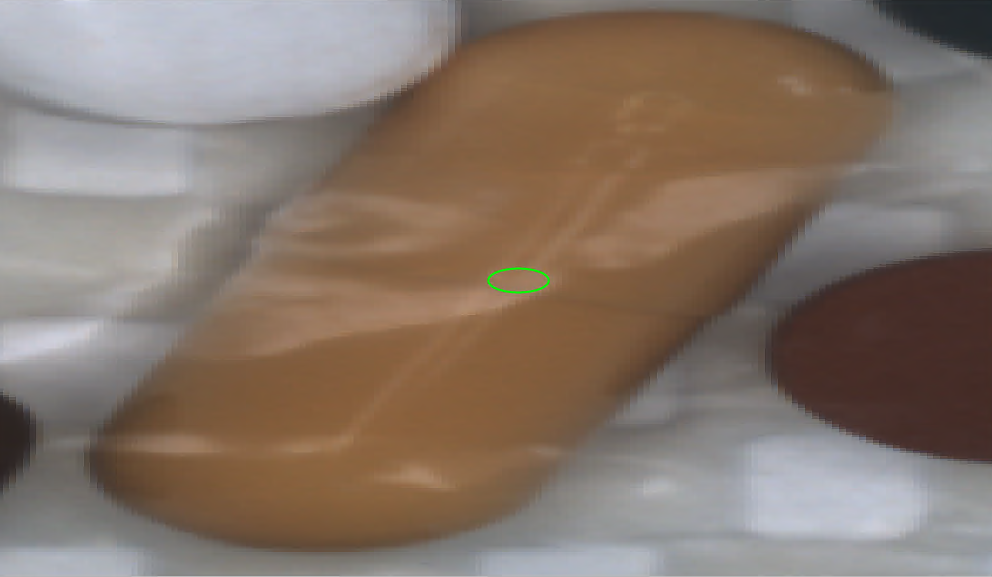
\includegraphics[width=\textwidth]{figures/chap32_watershed_application1.png}
		\caption{
			Plain cropped image with the object and the cursor with a foreground marker (green).\\
		} \label{fig:ch3:sec3:application1}
	\end{subfigure}
	\hfill
	\begin{subfigure}[t]{0.45\textwidth}
		\centering
		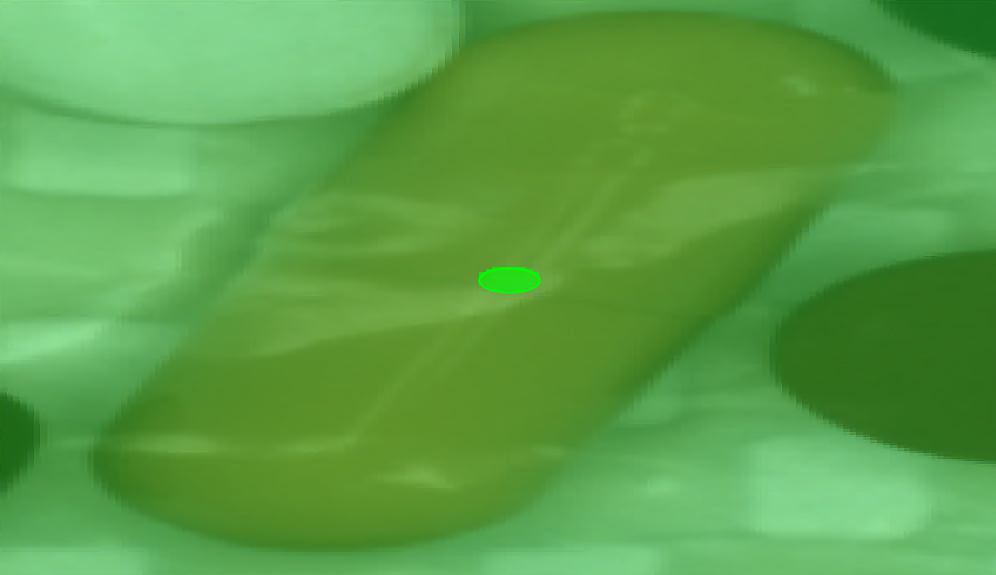
\includegraphics[width=\textwidth]{figures/chap32_watershed_application2.png}
		\caption{
			A foreground marker (green) is set and due to the absence of any background marker, the whole image is segmented as foreground.
		} \label{fig:ch3:sec3:application2}
	\end{subfigure}
	\\
	\begin{subfigure}[t]{0.45\textwidth}
		\centering
		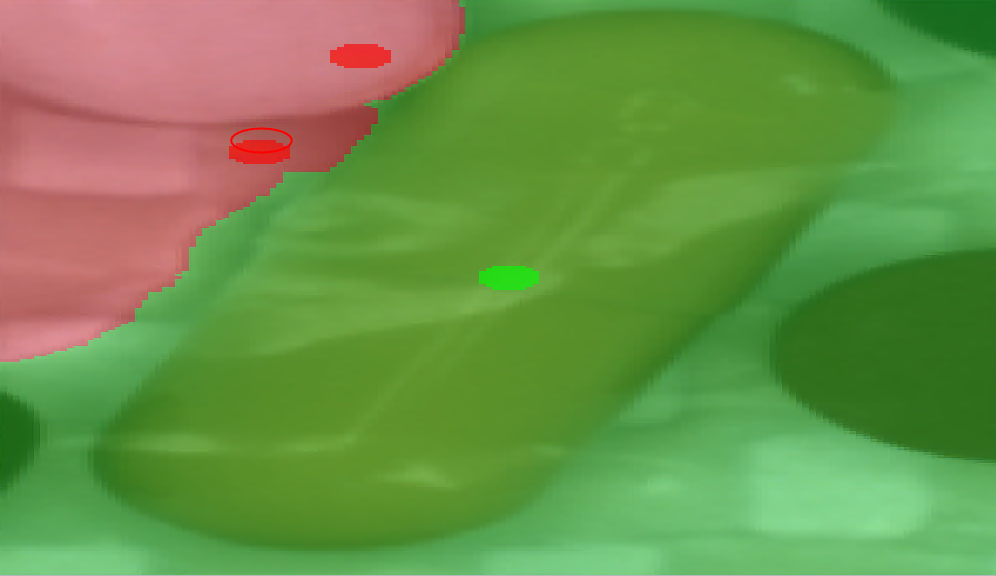
\includegraphics[width=\textwidth]{figures/chap32_watershed_application3.png}
		\caption{
			Two background markers (red) are set and the segmentation differentiates between fore- and background.\\
		} \label{fig:ch3:sec3:application3}
	\end{subfigure}
	\hfill
	\begin{subfigure}[t]{0.45\textwidth}
		\centering
		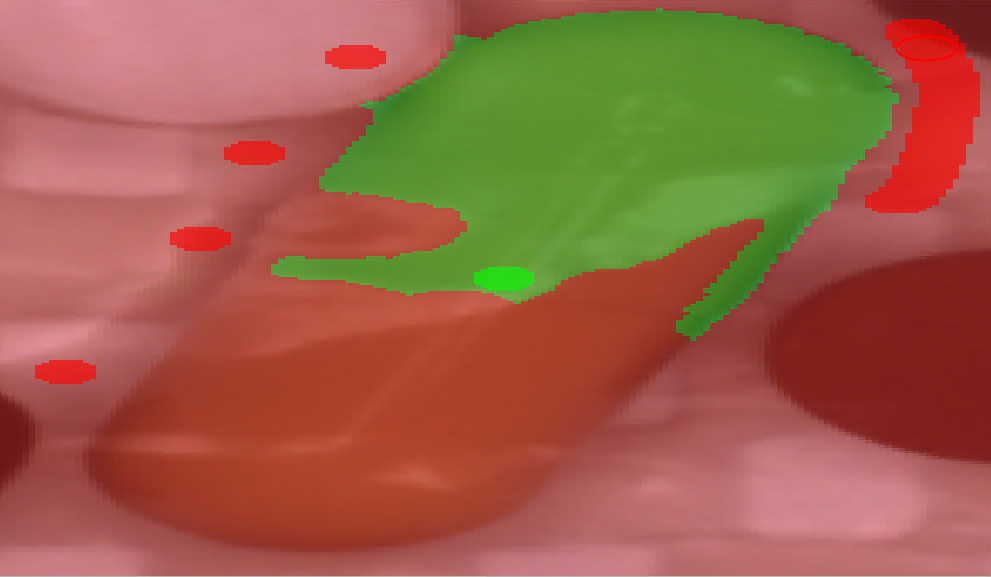
\includegraphics[width=\textwidth]{figures/chap32_watershed_application4.png}
		\caption{
			Additional background markers are set by two clicks and one stroke. 
			This results in a large area of the pill segmented as background.
		} \label{fig:ch3:sec3:application4}
	\end{subfigure}
	\\
	\begin{subfigure}[t]{0.45\textwidth}
		\centering
		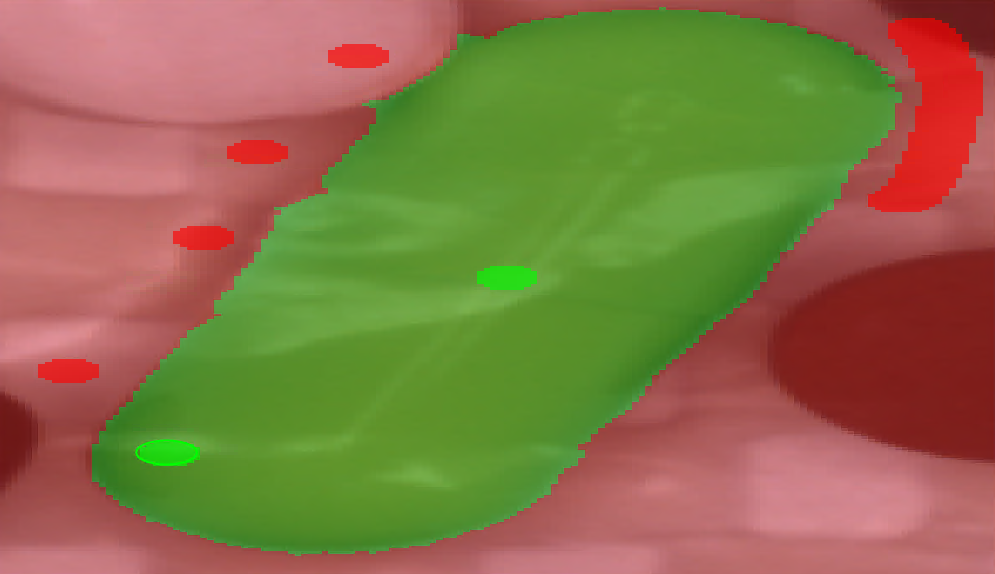
\includegraphics[width=\textwidth]{figures/chap32_watershed_application5.png}
		\caption{
			An additional foreground marker is set, which leads to a well segmented object.
		} \label{fig:ch3:sec3:application5}
	\end{subfigure}
	\hfill
	\begin{subfigure}[t]{0.45\textwidth}
		\centering
		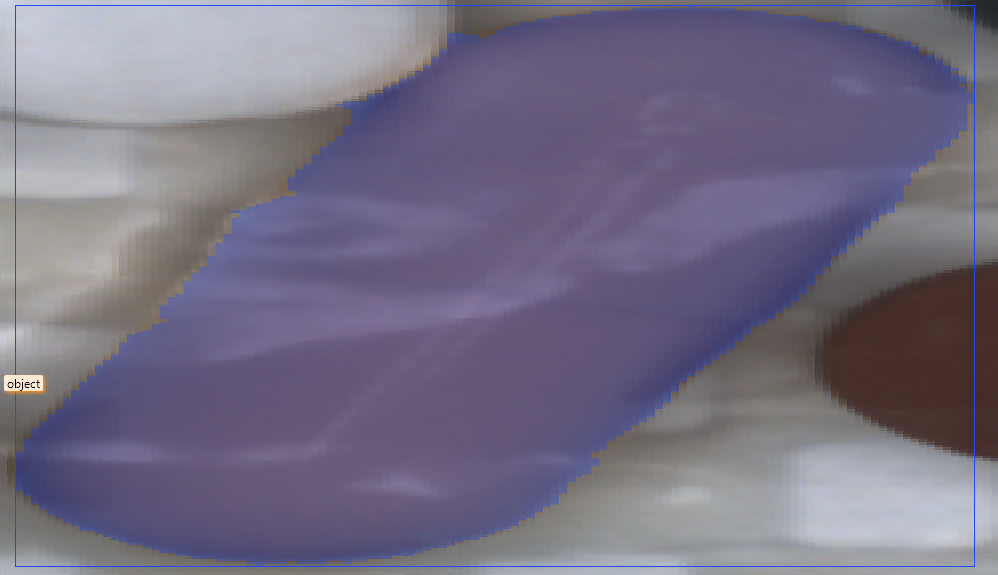
\includegraphics[width=\textwidth]{figures/chap32_watershed_application6.png}
		\caption{
			The final segmentation result.\newline	
		} \label{fig:ch3:sec3:application6}
	\end{subfigure}
	\caption [Watershed User Interaction]{
		Application of watershed segmentation on the image of a medical pill by setting fore- and background markers.
		The segmentation is based on two clicks on the foreground, four clicks and one stroke on the background.
	} \label{fig:ch3:sec2:application}
\end{figure}